\subsubsection{Caso d'uso UC8.2.5: Modifica domanda a ordinamento di immagini}
\label{UC8.2.5}
	\begin{figure}[ht]
		\centering
			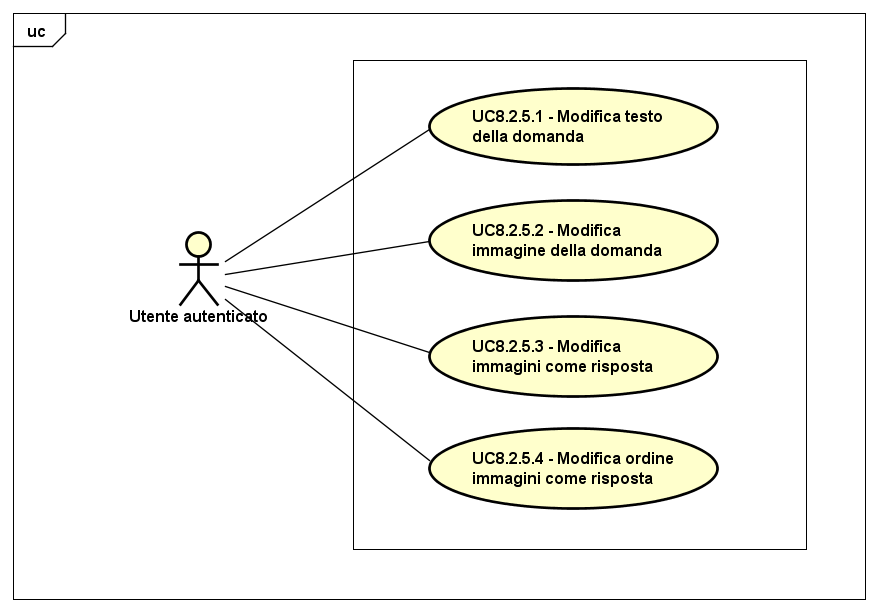
\includegraphics[scale=0.45,keepaspectratio]{UML/UC8_2_5.png}
		\caption{UC8.2.5: Modifica domanda a ordinamento di immagini}
	\end{figure}
\begin{itemize}
	\item\textbf{Attori}: utente autenticato, utente autenticato pro;
	\item\textbf{Descrizione}: l'attore può utilizzare la procedura guidata per la modifica di una domanda a ordinamento di immagini;
	\item\textbf{Precondizione}: il sistema ha ricevuto dall'attore la domanda da modificare; 
	\item \textbf{Postcondizione}: l'attore ha modificato una domanda a ordinamento di immagini;
	\item\textbf{Scenario principale}: 
	\begin{itemize}
		\item L'attore può modificare il testo della domanda (UC8.2.5.1);
		\item L'attore può modifica l'immagine relativa al testo della domanda (UC8.2.5.2);
		\item L'attore può modificare le immagini della sequenza che costituirà la risposta (UC8.2.5.3);
		\item L'attore può modifica l'ordine corretto delle immagini che costituiscono la risposta (UC8.2.5.4).
	\end{itemize}
\end{itemize}

\subsubsection{Caso d'uso UC8.2.5.1: Modifica testo della domanda}
\begin{itemize}
	\item\textbf{Attori}: utente autenticato, utente autenticato pro;
	\item \textbf{Descrizione}: l'attore può modificare il testo della domanda;
		\item
			\textbf{Precondizione}: il sistema mostra la funzionalità di modifica di una domanda a ordinamento di immagini; 
		\item
			\textbf{Postcondizione}: l'attore ha modificato il testo della domanda;
		\item
			\textbf{Scenario principale}: l'attore modifica il testo della domanda.	
	\end{itemize}

\subsubsection{Caso d'uso UC8.2.5.2: Modifica immagine della domanda}
\begin{itemize}
	\item\textbf{Attori}: utente autenticato, utente autenticato pro;
	\item \textbf{Descrizione}: l'attore può modificare l'immagine relativa al testo della domanda;
		\item
			\textbf{Precondizione}: il sistema mostra la funzionalità di modifica di una domanda di ordinamento immagini; 
		\item
			\textbf{Postcondizione}: l'attore ha modificato l'immagine relativa al testo della domanda;
		\item
			\textbf{Scenario principale}: l'attore modifica l'immagine relativa al testo della domanda. 	
	\end{itemize}

\subsubsection{Caso d'uso UC8.2.5.3: Modifica immagini come risposta}
\begin{itemize}
	\item\textbf{Attori}: utente autenticato, utente autenticato pro;
	\item\textbf{Descrizione}: l'attore può modificare le immagini che costituiscono la risposta alla domanda sostituendole con delle altre;
	\item\textbf{Precondizione}: il sistema mostra la funzionalità di modifica di una domanda di ordinamento immagini;  
	\item \textbf{Postcondizione}: l'attore ha inserito nuove immagini come risposta alla domanda;
	\item\textbf{Scenario principale}: l'attore sostituisce le immagini presenti come risposta alla domanda con delle altre.
\end{itemize}

\subsubsection{Caso d'uso UC8.2.5.4: Modifica ordine immagini come risposta}
\begin{itemize}
	\item\textbf{Attori}: utente autenticato, utente autenticato pro;
	\item\textbf{Descrizione}: l'attore può modificare l'ordine corretto delle immagini che rappresenta la soluzione della domanda;
	\item\textbf{Precondizione}: il sistema mostra la funzionalità di modifica di una domanda di ordinamento immagini; 
	\item \textbf{Postcondizione}: l'attore ha modificato l'ordine delle immagini che costituiscono la risposta alla domanda;
	\item\textbf{Scenario principale}: l'attore modifica l'ordine delle immagini che costituiscono la risposta alla domanda.
\end{itemize}
